\chapter{Model SGSTM}
\label{cap:model:sgstm}
\glsaddchap{not:sgstm}%%secció d'operacions
\glsreset{SGSTM}

En aquest capítol es defineix un model dels \glspl{SGSTM}, els quals
emmagatzemen sèries temporals de forma resumida i compacta. Aquest
model s'estructura en un objecte principal que són les \emph{sèries
  temporals multiresolució}, les quals es defineixen com a conjunts de
\emph{subsèries resolució} formades per \emph{discs} i \emph{buffers},
i utilitza els objectes de sèries temporals i mesures descrits en el
model de \gls{SGST}.  El model es dissenya en tres parts.

\begin{itemize}
\item Primer, es defineix el model d'estructura de les dades, és a
  dir, la forma que prenen els buffers, els discs, les subsèries
  resolució, les sèries temporals multiresolució i les bases de dades
  de sèries temporals multiresolució.

\item Segon, es defineix el model d'operacions sobre les dades, és a
  dir, els operadors bàsics que permeten modelar el comportament i la
  manipulació de bases de dades multiresolució.

\item Tercer, s'expliquen amb més detall les funcions específiques del
  model que permeten agregar diferents atributs de les sèries
  temporals per a obtenir les multiresolucions. Les funcions
  d'agregació d'atributs són requerides pel model però en són
  independents.
\end{itemize}




\section{Model estructural de dades}


Els objectes estructurals principals d'un \gls{SGSTM}, els quals es
defineixen en aquesta secció, són els següents:
\begin{itemize}
\item Buffer
\item Disc
\item Subsèrie resolució
\item Sèrie temporal multiresolució
\item Esquema de multiresolució
\end{itemize}


Resumint, una base de dades multiresolució és una solució
d'emmagatzematge per a sèries temporals en què la informació de
cadascuna es distribueix mitjançant diferents resolucions
temporals. Així, una base de dades multiresolució és un contenidor de
sèries temporals multiresolució on cadascuna és una subsèrie resolució
formada per una relació d'un buffer amb un disc. Cada sèrie temporal
multiresolució té un esquema de multiresolució que indica de quina
manera s'ha de resumir la informació i calcular les resolucions.

\begin{figure}[tp]
\centering
\begin{tikzpicture}
 \tikzset{
        myarrow/.style={->, >=latex',  thick},
      }
      

  \node[rectangle,draw,minimum height=6cm,minimum width=9cm] (m) {};
  \draw[shift=( m.south west)]   
  node[above right] {base de dades multiresolució};


  %discmig
  \node (m.center) (discr1) {...};

  %discr
  
  \node[ellipse,draw,minimum height=3.5cm,minimum width=2.5cm,alias=discr0] [left=of discr1] {};
  \node[above=0cm of discr0.north] {R0};
  \node[below=0cm of discr0] {disc resolució};

  \node[cylinder, draw, shape border rotate=90, aspect=0.25,alias=buffer0] [below=3mm of discr0.north] {buffer};
  \node[circle, draw,alias=disc0]  [above=3mm of discr0.south] {disc} ;
  \draw [->] (disc0.center)++(.4:.4cm) arc(0:180:.4cm);
  \draw[myarrow] (buffer0.bottom) -- (disc0.north);


  %discrd

  \node[ellipse,draw,minimum height=3.5cm,minimum width=2.5cm,alias=discrd] [right=of discr1] {};
  \node[above=0cm of discrd] {Rd};
  \node[below=0cm of discrd] {disc resolució};

  \node[cylinder, draw, shape border rotate=90, aspect=0.25,alias=bufferd] [below=3mm of discrd.north] {buffer};
  \node[circle, draw,alias=discd]  [above=3mm of discrd.south] {disc} ;
  \draw [->] (discd.center)++(.4:.4cm) arc(0:180:.4cm);
  \draw[myarrow] (bufferd.bottom) -- (discd.north);



  %mesura 
  \node[above=1cm of m.north] (m0) {};

  \draw[myarrow] (m0) -- (m.north) 
  node[right,midway] {mesura};

  \draw[myarrow] (m.north) -- (buffer0);
  \draw[myarrow] (m.north) -- (bufferd);
  \draw[myarrow] (m.north) -- (discr1);

\end{tikzpicture}
\caption{Arquitectura d'una base de dades multiresolució}
\label{fig:model:bdstm}
\end{figure}




Aquests objectes defineixen l'arquitectura d'una base de dades
multiresolució com es pot veure a la \autoref{fig:model:bdstm}.  Una
sèrie temporal multiresolució és una co\l.lecció de subsèries
resolució, les quals acumulen temporalment mesures en un buffer a on
són processades i finalment emmagatzemades en un disc. Aquest
processament té per objectiu canviar els intervals de temps entre les
mesures per tal de compactar la informació de les sèries temporals i
emmagatzemar-la en forma de subsèries temporals amb diferents
resolucions distribuïdes en els discs. Els discs tenen la mida
limitada i només poden contenir un nombre fixat de mesures; quan no hi
ha més capacitat cal eliminar mesures.  En síntesi, una base de dades
multiresolució té la mida fixada i les sèries temporals hi queden
emmagatzemades en forma de multiresolució, és a dir a trossos com a
subsèries temporals.


En aquesta secció només es defineixen els conceptes referents a
l'estructura del model i al final s'ofereixen alguns exemples amb
valors concrets. Aquesta estructura, però, requereix uns operadors
específics per a emmagatzemar-hi i consolidar-hi les mesures, els
quals es defineixen a
l'\autoref{sec:model:sgstm-estructurals}. També requereix unes
funcions per a agregar els atributs d'una sèrie temporal, les quals
es defineixen a la \autoref{sec:model:agregador}.




\subsection{Buffer}\label{sec:model:buffer}



Un buffer és un contenidor d'una sèrie temporal que s'ocupa
d'emmagatzemar les mesures pendents de ser consolidades i de
consolidar-les en funció d'unes característiques definides
prèviament. Les mesures es poden eliminar un cop s'han consolidat.

La consolidació d'un buffer té com a objectiu regularitzar la sèrie
temporal a un període de mostreig constant
(v.~\autoref{def:st:regular} i \autoref{sec:sgst:regularitzacio}).
Així, els paràmetres d'un buffer són: el període temporal de
consolidació, que anomenen pas de consolidació; l'instant inicial de
consolidació, que s'expressa com el darrer instant de temps de
consolidació; i la funció que extreu les
característiques de la consolidació, el càlcul de la qual es delega al
que anomenem funció d'agregació d'atributs.


\begin{definition}[Buffer]
  Definim \emph{buffer} com el tuple
  \glsdispdef{not:buffer}{$(S_B,\tau,\delta,f)$}, en què
  \glsdispdef{not:sgstm:sb}{$S_B$} és una sèrie temporal pendent de
  ser consolidada, \glsdispdef{not:sgstm:tau}{$\tau$} és el darrer
  instant de temps de consolidació,
  \glsdispdef{not:sgstm:delta}{$\delta$} és una durada de temps que
  indica el pas de consolidació i \glsdispdef{not:sgstm:f}{$f$} és una
  funció d'agregació d'atributs.
\end{definition}

La consolidació d'una sèrie temporal s'inicia en un instant de temps
concret, $\tau$, i ocorre a cada pas de consolidació, $\delta$. Amb la
finalitat d'establir els intervals de consolidació de la sèrie
temporal, es defineix un buffer inicial.

\begin{definition}\label{def:model:buffer_buit}
  Definim buffer inicial o buffer buit com el buffer $B_{\emptyset} =
  (\emptyset,\tau_0, \delta, f)$, el qual conté una sèrie temporal
  buida, l'instant de temps inicial de consolidació, el pas de
  consolidació i una funció d'agregació d'atributs.
\end{definition}

A partir del buffer buit es poden conèixer tots els instants de temps
de consolidació del buffer, els quals seran $\tau_0+k\delta,
k\in\glssymbol{not:N}$. Aquests instants de temps de consolidació
també defineixen els intervals de temps de consolidació del buffer de
la forma $i=[\tau,\tau+\delta]$. La consolidació de la sèrie temporal
$S_B$ d'un buffer en un interval de temps $i$ dóna com a resultat una
mesura $m'=(t,v)$ calculada a partir de la funció d'agregació
d'atributs $m' = f (S, i)$. Més endavant a la
\autoref{sec:model:agregador} detallem el concepte de funció
d'agregació d'atributs.


\begin{figure}[tp]
  \centering
   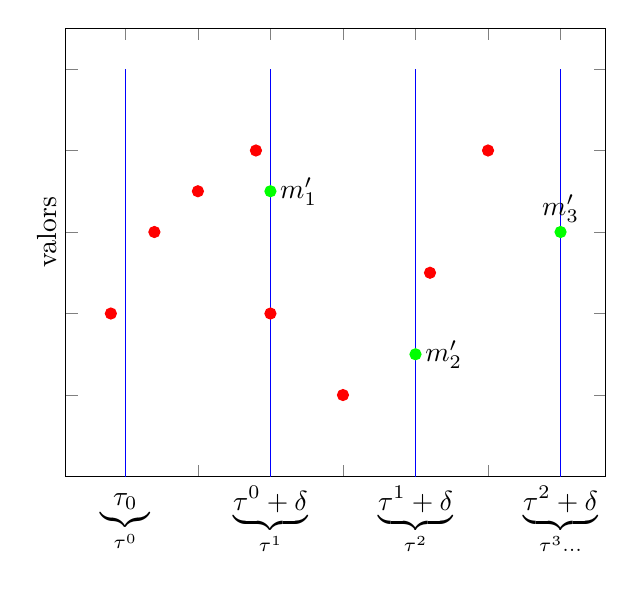
\begin{tikzpicture}
    \begin{axis}[
        ymin = 0,
        yticklabels= {,,,,valors},
        y tick label style = {rotate=90,anchor=south},
        xticklabels={,,$\underbrace{\tau_{0}\vphantom{\delta}}_{\tau^0}$,,$\underbrace{\tau^0+\delta}_{\tau^1}$,,$\underbrace{\tau^1+\delta}_{\tau^2}$,,$\underbrace{\tau^2+\delta}_{\tau^3 \ldots}$},
        ]
 
    \addplot[ycomb,blue] coordinates {
        (20,10)
        (30,10)
        (40,10)
        (50,10)
    }; 

    \addplot[red,only marks, mark = *] coordinates {
        (19,4)
        (22,6)
        (25,7)
        (29,8)
        (30,4)
        (35,2)
        (41,5)
        (45,8)
    };

          \addplot[only marks,mark=*,green] coordinates {
            (30,7)
            (40,3)
            (50,6)
          };

          \node[right] at (axis cs:30,7) {$m'_1$};
          \node[right] at (axis cs:40,3) {$m'_2$};
          \node[above] at (axis cs:50,6) {$m'_3$};
    \end{axis}
  \end{tikzpicture}

  \caption{Intervals de consolidació d'un buffer}
  \label{fig:sgstm:consB}
\end{figure}




A la \autoref{fig:sgstm:consB} es mostra un exemple de sèrie temporal
les mesures de la qual es mostren amb punts vermells, en línies blaves
verticals s'indiquen els intervals de consolidació d'un buffer sobre
aquesta sèrie temporal, i les mesures consolidades es mostren amb
punts verds.  Sigui $\tau_0$ l'instant inicial de consolidació, el
primer instant de consolidació $\tau$, anomenant-lo $\tau^0$ com el
primer valor que pren, és $\tau^0=\tau_0$. El següent valor que
prendrà és $\tau^1=\tau^0+\delta$ i així successivament.  Per tant el
primer interval de consolidació és $i^0=[\tau^0,\tau^1]$. Quan es
consolida el buffer per aquest interval, el darrer instant de
consolidació esdevé $\tau^1$ i es calcula una mesura
$m'_1=f(S,[\tau^0,\tau^1])$; la qual per facilitar la comprensió podem
assumir de moment que és el resultat de calcular una agregació sobre
les mesures en l'interval $[\tau^0,\tau^1]$. De la mateixa manera es
calculen les mesures consolidades $m_2'$ i $m_3'$.




\subsection{Disc}\label{sec:model:disc}


Un disc és un contenidor d'una sèrie temporal regular amb un nombre
acotat de mesures. En arribar al nombre màxim de mesures permeses,
cada cop que s'afegeix una mesura nova s'elimina la mesura mínima de
la sèrie temporal.  Així doncs, un disc és semblant a una cua
\emph{First In First Out}, en què el primer d'arribar és el
primer de sortir.

\begin{definition}[Disc]
  Definim \emph{disc} com el tuple \glsdispdef{not:disc}{$(S_D,k)$},
  en què \glsdispdef{not:sgstm:sd}{$S_D$} és una sèrie temporal
  regular i \glsdispdef{not:sgstm:k}{$k\in\glssymbol{not:N}$} és el
  cardinal màxim de $S_D$.
\end{definition}

A l'inici, un disc no conté mesures però cal que estigui caracteritzat
pel cardinal màxim. Amb aquesta finalitat es defineix un disc inicial.

\begin{definition}\label{def:model:disc_buit}
  Definim disc inicial o disc buit com el disc $D_{\emptyset} =
  (\emptyset,k)$, el qual conté una sèrie temporal buida i el cardinal
  màxim que podrà prendre $S_D$.
\end{definition}



\subsection{Subsèrie resolució}\label{sec:model:subserie-resolucio}


Una subsèrie resolució és una parella de disc i buffer. En el
buffer hi ha la part d'una sèrie temporal a regularitzar i en el disc
hi ha l'altra part ja regularitzada, amb un nombre afitat de
mesures. A l'acció de regularitzar l'anomenem consolidar en coherència
amb el concepte descrit pels buffers. 



\begin{definition}[Subsèrie resolució]
  Definim \emph{subsèrie resolució} com el tuple
  \glsdispdef{not:subserieresolucio}{$(B,D)$}, en què $B$ és un buffer i $D$
  és un disc.
\end{definition}
 
La \autoref{def:model:buffer_buit} de buffer buit i la
\autoref{def:model:disc_buit} de disc buit indueixen a una definició
de subsèrie resolució buida.  

\begin{definition}\label{def:model:subserie_resolucio_buida}
  Definim subsèrie resolució buida com la subsèrie resolució $R_{\emptyset}
  = (B_{\emptyset},D_{\emptyset})$, la qual conté un buffer buit i un
  disc buit.
\end{definition}


Les subsèries resolució es consoliden seguint els criteris del seu
buffer i emmagatzemant al seu disc la mesura que resulta de la
consolidació. Així, els paràmetres del buffer i del disc d'una
subsèrie resolució ($\tau_0, \delta, f, k$) caracteritzen la resolució
de la subsèrie temporal $S_D$ que finalment queda emmagatzemada.  A la
\autoref{fig:sgstm:bdsubserie} es mostra un esquema semblant a la
\autoref{fig:model:bdstm} on es veu una subsèrie resolució amb la
relació d'aquests paràmetres entre el buffer i el disc, llevat de
$\tau_0$ que és difícil de representar.


\begin{figure}[tp]
  \centering
  
\begin{tikzpicture}
 \tikzset{
        myarrow/.style={->, >=latex',  thick},
      }
      

  %discr
  
  \node[ellipse,draw,minimum height=3.5cm,minimum width=2.5cm,alias=discr0]  {};

  \node[cylinder, draw, shape border rotate=90, aspect=0.25,alias=buffer0] [below=3mm of discr0.north] {$f$};
  \node[circle, draw,alias=disc0,minimum width=1.2cm]  [above=3mm of discr0.south] {$\delta$} ;
  \draw [->] (disc0.center)++(.2:.2cm) arc(0:180:.2cm);
  \draw[myarrow] (buffer0.bottom) -- (disc0.north);

  \node[circle,minimum width=9mm] (d0boles) [below=0mm of disc0.center,anchor=center] {};
  \node[below=0mm of d0boles.north,anchor=center] {$\circ$};
  \node[below=0mm of d0boles.east,anchor=center] {$\circ$};
  \node[below=0mm of d0boles.south,anchor=center] {$\circ$};
  \node[below=0mm of d0boles.west,anchor=center] {$\circ$};

  \node[below=0mm of d0boles.east,anchor=south west] {$k)$};

%  \node[circle, draw,dotted,minimum width=1cm]  (disc0.center) {} ;
  \draw [dotted] (disc0.center)++(.5:.5cm) arc(0:360:.5cm);

\end{tikzpicture}
  \caption{Paràmetres d'una subsèrie temporal resolució}
  \label{fig:sgstm:bdsubserie}
\end{figure}



\subsection{Sèrie temporal multiresolució}


Una sèrie temporal multiresolució és un conjunt de subsèries resolució
que comparteixen l'entrada de mesures, les quals provenen d'una
mateixa sèrie temporal. Aquesta sèrie temporal queda regularitzada i
distribuïda en les diferents subsèries resolució amb paràmetres
diferents, tal com s'ha vist a la \autoref{fig:model:bdstm}


\begin{definition}[Sèrie temporal multiresolució]
  \label{def:sgstm:stm}
  Definim \emph{sèrie temporal multiresolució} com el conjunt de subsèries
  resolució \glsdispdef{not:seriemultiresolucio}{$M=\{R_0,\dotsc,R_d\}$}.
\end{definition}

A partir de la \autoref{def:model:subserie_resolucio_buida} de
subsèrie resolució buida és defineix la sèrie temporal multiresolució
buida.
 
\begin{definition}\label{def:model:st_multiresolucio_buit}
  Definim sèrie temporal multiresolució buida o inicial com el conjunt
  de subsèries resolució buides
  $M_{\emptyset}=\{R_{0_{\emptyset}},\dotsc,R_{d_{\emptyset}\}}$.
\end{definition}


Normalment, en una sèrie temporal multiresolució no hi ha dues
subsèries resolució amb la mateixa informació. És a dir, no hi dues
subsèries resolució el buffers de les quals tinguin alhora el mateix
pas de consolidació i funció d'agregació d'atributs: $\forall
R_i,R_j\in M, i\neq j : \delta_i \neq \delta_j \vee f_i \neq f_j$ on
$R_i = (B_i, D_i)$, $R_j = (B_j, D_j)$,
$B_i=(S_i,\tau_i,\delta_i,f_i)$ i $B_j=(S_j,\tau_j,\delta_j,f_j)$.



\subsubsection{Relació sèrie temporal multiresolució}

Una sèrie temporal multiresolució s'expressa com un conjunt i com a
tal és susceptible d'aplicar-hi els conceptes del model dels
\glspl{SGBDR}, a continuació expressem la forma de sèrie temporal
multiresolució seguint també el concepte de relació. 


Una sèrie temporal multiresolució és una
relació de buffers i discs. A cada parella buffer-disc l'anomenem
subsèrie resolució. Així doncs, una sèrie temporal multiresolució és
un conjunt de subsèries resolució.
Com a conjunt de subsèries resolució, una sèrie temporal multiresolució
s'observa com una relació de grau sis en què la capçalera conté els
atributs
\begin{itemize}
\item sèrie temporal del buffer ($S_B$),
\item sèrie temporal del disc ($S_D$),
\item darrer instant de consolidació ($\tau$),
\item pas de consolidació ($\delta$),
\item màxim cardinal del disc ($k$),
\item i funció d'agregació d'atributs ($f$).
\end{itemize}



Com ja s'ha comentat, una restricció habitual és que $\delta$ i $f$ no
estiguin repetits, és a dir que és una restricció que indica que els
atributs $\{\delta,f\}$ són la clau primària.  El predicat
corresponent a les sèries temporals multiresolució és similar a: «La
resolució amb pas de consolidació \emph{$\delta$} i funció d'agregació
\emph{$f$}, de la qual se n'emmagatzemarà com a màxim \emph{$k$}
mesures, s'ha consolidat amb la sèrie temporal \emph{$S_D$} per darrer
cop a l'instant \emph{$\tau$} i té pendent per consolidar la sèrie
temporal \emph{$S_B$}».



Així doncs observada com a relació, i tal com s'ha fet per a la forma
canònica de les sèries temporals
(v.~\autoref{def:sgst:forma-canonica}), podem escriure la forma
canònica d'una sèrie temporal multiresolució.
\begin{definition}[Forma canònica]
  Sigui $M=\{R_0,\dotsc,R_d\}$ una sèrie temporal multiresolució on
  cada subsèrie resolució $R_i =(B_i,D_i),
  B_i=(S_{B_i},\tau_i,\delta_i,f_i), D_i=(S_{D_i},k_i)$ té domini de
  sèrie temporal per les sèries temporals $S_{B_i}$ i $S_{D_i}$, de
  $\glssymbol{not:Rb}$ pels temps $\tau_i$ i $\delta_i$, de
  $\glssymbol{not:N}$ pel cardinal $k$, i de funció per a la funció
  d'agregació d'atributs; \glsdispdef{not:sgstm:canonica}{en la forma
    canònica} s'escriu com $ M = ( \{S_B: \text{sèrie temporal}, S_D:
  \text{sèrie temporal}, \tau: \glssymbol{not:Rb}, \delta:
  \glssymbol{not:Rb}, k: \glssymbol{not:N}, f: \text{funció}\}, \{ \{
  (S_B, S_{B_0}) , (S_D , S_{D_0}) , (\tau, \tau_0), (\delta,
  \delta_0), (k, k_0), (f, f_0) \} , \dotsc, \{ (S_B,
  S_{B_d}) , (S_D , S_{D_d}) , (\tau, \tau_d), (\delta,
  \delta_d), (k, k_d), (f, f_d) \} \} )$.
\end{definition}



De la mateixa manera que per a les sèries temporals, també escrivim
una sèrie temporal multiresolució de manera simplificada com el
conjunt de tuples $M = \{ (S_{B_0}, S_{D_0} , \tau_0, \delta_0, k_0,
f_0 ), \dotsc, (S_{B_d}, S_{D_d} , \tau_d, \delta_d, k_d, f_d ) \}$,
la qual es correspon amb la forma expressada inicialment a la
\autoref{def:sgstm:stm} amb els tuples de $B_i$ i $D_i$ units.  També
com amb les sèries temporals, les sèries temporals multiresolució es
poden visualitzar com a taules, cosa que mostrem en exemples
posteriors.






\subsection{Esquema de multiresolució}

Una sèrie temporal multiresolució té paràmetres que
s'han de configurar en el seu estat inicial: la quantitat de subsèries
resolucions i els paràmetres de cada una --pas de consolidació, funció
d'agregació d'atributs, darrer instant de consolidació i cardinal
màxim. Anomenem esquema de multiresolució a les configuracions
possibles d'aquests paràmetres.


En la forma canònica de les sèries temporals multiresolució es pot
observar més clarament que els atributs $\{\delta,\tau,f,k\}$ són els
paràmetres configurables al conjunt de tuples dels quals anomenem
esquema de multiresolució.
\begin{definition}[Esquema de multiresolució]
  \label{def:sgstm:esquema}
  Sigui $M=\{R_0,\dotsc,R_d\}$ una sèrie temporal multiresolució, el
  seu \glsdispdef{not:esquemaM}{esquema de multiresolució $e$} és la
  projecció dels atributs que constitueixen els paràmetres
  configurables:
  $e=\glssymbol{not:sgst:project}_{\{\delta,\tau,f,k\}}(M)$. Així,
  l'esquema de multiresolució de $M$ es pot expressar com la relació
  $e = \{ (\delta_0,\tau_0,f_0,k_0), \dotsc,
  (\delta_d,\tau_d,f_d,k_d)\}$, és a dir una relació amb la capçalera
  $\{\delta,\tau,f,k\}$.
\end{definition}


Per a cada sèrie temporal multiresolució es pot estudiar i manipular
l'esquema de multiresolució, la qual cosa mostrem amb més detall a
l'\autoref{sec:model:sgstm-manipulacio-esquema}.





\subsection{Exemples}


\begin{example} [Sèrie temporal multiresolució]
\label{ex:model:bdm1}%ATENCIÓ als canvis: les dades d'aquest exemple s'utilitzen en altres apartat.


Sèrie temporal multiresolució $M_1=\{R_1,R_2\}$ que té dues subsèries
resolució amb els paràmetres següents:
\begin{itemize}
\item La subsèrie resolució $R_1$ té un pas de consolidació de 5
  unitats de temps, una mida màxima de 4 mesures i una funció de
  consolidació de `mitjana' de les mesures.
\item La subsèrie resolució $R_2$ té un pas de consolidació de 10
  unitats de temps, una mida màxima de 3 mesures i una funció de
  consolidació de `mitjana' de les mesures.
\end{itemize}

\begin{figure}[tp]
\centering
%\usetikzlibrary{shapes,arrows,positioning}
\begin{tikzpicture}
 \tikzset{
        myarrow/.style={->, >=latex',  thick},
      }
      

  \node[rectangle,draw,minimum height=6cm,minimum width=9cm] (m) {};
  \draw[shift=( m.south west)]   
  node[above right] {base de dades multiresolució};


  %discmig
  \node (m.center) (discr1) {};

  %discr
  
  \node[ellipse,draw,minimum height=3.5cm,minimum width=2.5cm,alias=discr0] [left=of discr1] {};
  \node[above=0cm of discr0.north] {$R_0$};
  \node[below=0cm of discr0] {subsèrie resolució};

  \node[cylinder, draw, shape border rotate=90, aspect=0.25,alias=buffer0] [below=3mm of discr0.north] {mitjana};
  \node[circle, draw,alias=disc0,minimum width=1.2cm]  [above=3mm of discr0.south] {5} ;
  \draw [->] (disc0.center)++(.2:.2cm) arc(0:180:.2cm);
  \draw[myarrow] (buffer0.bottom) -- (disc0.north);

  \node[circle,minimum width=9mm] (d0boles) [below=0mm of disc0.center,anchor=center] {};
  \node[below=0mm of d0boles.north,anchor=center] {$\circ$};
  \node[below=0mm of d0boles.east,anchor=center] {$\circ$};
  \node[below=0mm of d0boles.south,anchor=center] {$\circ$};
  \node[below=0mm of d0boles.west,anchor=center] {$\circ$};


  %discrd

  \node[ellipse,draw,minimum height=3.5cm,minimum width=2.5cm,alias=discrd] [right=of discr1] {};
  \node[above=0cm of discrd] {$R_1$};
  \node[below=0cm of discrd] {subsèrie resolució};

  \node[cylinder, draw, shape border rotate=90, aspect=0.25,alias=bufferd] [below=3mm of discrd.north] {mitjana};
  \node[circle, draw,alias=discd,minimum width=1.2cm]  [above=3mm of discrd.south] {10} ;
  \draw [->] (discd.center)++(.3:.3cm) arc(0:180:.3cm);
  \draw[myarrow] (bufferd.bottom) -- (discd.north);

  \node[circle,minimum width=9mm] (d1boles) [below=0mm of discd.center,anchor=center] {};
  \node[below=0mm of d1boles.north,anchor=center] {$\circ$};
  \node[below=0mm of d1boles.south east,anchor=center] {$\circ$};
  \node[below=0mm of d1boles.south west,anchor=center] {$\circ$};


  %mesura 
  \node[above=1cm of m.north] (m0) {};

  \draw[myarrow] (m0) -- (m.north) 
  node[right,midway] {mesura};

  \draw[myarrow] (m.north) -- (buffer0);
  \draw[myarrow] (m.north) -- (bufferd);


\end{tikzpicture}
\caption{Arquitectura de la base de dades multiresolució particular
  per l'\autoref{ex:model:bdm1}}
\label{fig:model:ex1}
\end{figure}

L'arquitectura de la base de dades que conté aquesta sèrie temporal
multiresolució es pot veure a la \autoref{fig:model:ex1}. 
 L'esquema
de multiresolució que correspon als instants de consolidació, des de 0
fins a 30, és el següent:
\begin{itemize}
\item La subsèrie resolució $R_1$ serà consolidada en els instants 5,
  10, 15, 20, 25 i 30.
\item La subsèrie resolució $R_2$ serà consolidada en els instants 10,
  20 i 30.
\end{itemize}


Iniciem la base de dades a l'instant de temps 0, instant en el qual la
sèrie temporal multiresolució és $M_1^0 = \{ ( \{\} , \{\} , 0 , 5 ,4
, \text{mitjana} ) , ( \{\} , \{\} , 0 , 10 ,3 , \text{mitjana} ) \}$;
és a dir amb les sèries temporals buides i els darrers instants de
consolidació iniciats a 0.




A continuació, afegim a la sèrie temporal multiresolució les mesures
de la sèrie temporal $S_1=\{
(1,0),(5,0),(8,0),(10,0),(14,0),(19,0),(22,0),(26,0),(29,0) \}$. Tots
els valors valen zero per tal de centrar la comprensió de l'exemple en
l'estructura de temps de consolidació; pel que fa a exemples
d'agregació de valors es poden veure amb més detall a la
secció~\ref{sec:model:agregador}.


Si consolidem la sèrie temporal multiresolució cada cop que sigui
consolidable, és a dir en els instants que marca l'esquema de
multiresolució, a l'instant 29 després d'haver inserit la darrera
mesura la sèrie temporal multiresolució és $M_1^{29} = \{ (
\{(26,0),(29,0)\},\{(10,0),(15,0),(20,0),(25,0)\}, 25 , 5 ,4 ,
\text{mitjana} ), ( \{(22,0),(26,0),(29,0)\}, \{(10,0),(20,0)\},
20 , 10 ,3 , \text{mitjana} ) \}$.  Aquesta sèrie temporal
multiresolució es mostra a la \autoref{fig:model:stm} en forma de
taula.


Es pot observar que als buffers hi ha emmagatzemades les mesures
pendents de consolidar per a cada subsèrie i als discs les darreres
mesures consolidades:
\begin{itemize}
\item Per a la subsèrie resolució $R_1$ hi ha pendent de consolidar
  l'interval de temps $[25,30]$ i al disc hi ha emmagatzemades les 4
  mesures màximes permeses; és a dir que la que s'havia consolidat a
  l'instant $5$ ja s'ha perdut.
\item Per a la subsèrie resolució $R_2$ hi ha pendent de consolidar
  l'interval de temps $[20,30]$ i al disc hi ha emmagatzemades 2
  mesures. El disc encara no ha arribat al cardinal màxim $k=3$ a
  causa que la base de dades s'ha iniciat a l'instant $0$ i la primera
  consolidació d'aquesta subsèrie ha estat a l'instant $10$.
\end{itemize}




\begin{figure}[tp]
  \centering
  \begin{tabular}{|c|c|c|c|c|c|}
    \multicolumn{2}{c}{$M_1^{29}$} \\ \hline
    $S_B$  & $S_D$ & $\tau$ & $\delta$ & $k$ & $f$ \\ \hline
      \begin{tabular}{|c|c|}
         \hline
         $t$  & $v$ \\ \hline
         26  & 0 \\
         29 & 0 \\\hline
       \end{tabular} & 
      \begin{tabular}{|c|c|}
         \hline
         $t$  & $v$ \\ \hline
         10  & 0 \\
         15  & 0 \\
         20 & 0 \\ 
         25 & 0 \\\hline
       \end{tabular} 
       & 25 & 5  & 4 & mitjana  \\ \hline
       \begin{tabular}{|c|c|}
         \hline
         $t$  & $v$ \\ \hline
         22  & 0 \\
         26  & 0 \\
         29 & 0 \\\hline
       \end{tabular} & 
      \begin{tabular}{|c|c|}
         \hline
         $t$  & $v$ \\ \hline
         10  & 0 \\
         20  & 0 \\\hline
       \end{tabular}  
       & 20 & 10 & 3 & mitjana  \\ \hline
  \end{tabular}
  \caption{Taula d'una sèrie temporal multiresolució a l'instant $29$}
  \label{fig:model:stm}
\end{figure}

\end{example}


\begin{example} [Sèrie temporal multiresolució amb vistes]
  \label{ex:model:bdm-vistes}

  En el model \gls{SGBDR} molt sovint s'utilitzen vistes per a
  agrupar informació de vàries relacions, per a mostrar-ne una part,
  etc. Una vista és una variable relació virtual derivada d'una
  expressió relacional \parencite{date13}. En aquest exemple mostrem
  la mateixa sèrie temporal multiresolució de
  l'\autoref{ex:model:bdm1} però organitzada amb forma de vistes
  relacionals.


  Siguin una relació de sèries temporals i noms $M_2^{\text{series}}=
  ((S':\text{nom},S:\text{sèrie temporal}),\{
  (S_{B1},\{(26,0),(29,0)\}), (S_{B2},\{(22,0),(26,0),(29,0)\}),
  (S_{D1},\{(10,0), (15,0), (20,0), (25,0)\}), (S_{D2},\{(10,0),
  (20,0)\} )\})$ i una sèrie temporal multiresolució amb noms com a
  domini dels atributs de sèries temporals $M_2^{\text{noms}}=
  ((S'_B:\text{nom},S'_D:\text{nom}, \tau:\glssymbol{not:Rb},
  \delta:\glssymbol{not:Rb}, k:\glssymbol{not:N}, f:\text{funció} ),\{
  (S_{B1},S_{D1},25 ,5 ,4 ,\text{mitjana} ), ( S_{B2},S_{D2},20 , 10
  ,3 , \text{mitjana} ) \})$, les quals es mostren a la
  \autoref{fig:model:stm:vistes}, la vista de la sèrie temporal
  multiresolució es defineix com
  \begin{align*}
    \text{vista } M_2 =& \glssymbol{not:sgst:project}_{\text{tots llevat } \{S_B',S_D'\} } \big( M_2^{\text{noms}} \glssymbol{not:sgst:join} (\glssymbol{not:sgst:rename}_{\{S'/S_B', S/S_B\}} M_2^{\text{series}}) \\
    & \glssymbol{not:sgst:join} (\glssymbol{not:sgst:rename}_{\{S'/S_D',
      S/S_D\}} M_2^{\text{series}} )\big)
  \end{align*}

  aplicant les operacions relacionals de reanomena, junció i
  projecció.



  \begin{figure}[tp]
    \centering
    \begin{tabular}{|c|c|c|c|c|c|}
      \multicolumn{2}{c}{$M_2^{\text{noms}}$} \\ \hline
      $S'_B$  & $S'_D$ & $\tau$ & $\delta$ & $k$ & $f$ \\ \hline
      $S_{B1}$ & $S_{D1}$ & 25 & 5  & 4 & mitjana  \\
      $S_{B2}$ & $S_{D2}$ & 20 & 10 & 3 & mitjana  \\ \hline
    \end{tabular}\qquad
    \begin{tabular}{|c|c|c|}
      \multicolumn{3}{c}{$M^{\text{series}}_{2}$} \\ \hline
      \multirow{2}{*}{$S'$}  &  \multicolumn{2}{c|}{$S$} \\ \cline{2-3}
      & $t$      & $v$  \\ \hline
      \multirow{2}{*}{$S_{B1}$} 
      & 26 & 0 \\ 
      & 29 & 0 \\ \hline
      \multirow{3}{*}{$S_{B2}$} 
      & 22 & 0 \\ 
      & 26 & 0 \\ 
      & 29 & 0 \\ \hline
      \multirow{4}{*}{$S_{D1}$} 
      & 10 & 0 \\ 
      & 15 & 0 \\ 
      & 20 & 0 \\ 
      & 25 & 0 \\ \hline
      \multirow{2}{*}{$S_{D2}$} 
      & 10 & 0 \\ 
      & 20 & 0 \\ \hline
    \end{tabular}
    \caption{Taula d'una sèrie temporal multiresolució amb vistes
      relacionals}
    \label{fig:model:stm:vistes}
  \end{figure}


  D'aquesta manera $M_2$ té els mateixos valors que la $M_1$ definida
  a l'exemple anterior és a dir que es visualitza amb la mateixa taula
  que la de la \autoref{fig:model:stm}; observant només el resultat de
  $M_2$ no es pot distingir que és una vista. Així doncs, les vistes
  permeten organitzar una sèrie temporal multiresolució de forma més
  còmoda i a més, tal com descriu \textcite{date13}, mantenint que
  totes les operacions i propietats que són d'aplicació a les
  relacions ho són també a les seves vistes.


%S'observa que per tal de complir amb les propietats de les relacions, totes les sèries temporals dels buffers han de ser del mateix tipus, és a dir tenir la mateixa capçalera. El mateix succeeix amb les sèries temporals dels discs. (Vegeu els exemples de la secció \ref{par:model:exemple-relvalues} sobre valors relació). No obstant les mesures que entren a la base de dades provenen de la mateixa sèrie temporal i per tant les sèries temporals emmagatzemades sempre seran del mateix tipus.



\end{example}


\begin{example} [Sèrie temporal multiresolució amb desfasaments]
\label{ex:model:bdm-desfasaments}

A l'\autoref{ex:model:bdm1} s'ha mostrat una sèrie temporal
multiresolució en què la consolidació de les dues subsèries obeeix
a la mateixa funció d'agregador d'atributs $f$. En aquest exemple
treballem amb els mateixos valors que a l'\autoref{ex:model:bdm1} però
ara canviem la funció de la segona subsèrie resolució per un agregador
amb desfasament; és a dir que cada cop que consolida retorna una
mesura amb un retard d'una certa durada. Aquest nou agregador que
anomenem \emph{mitjanad5} també fa la mitjana però amb un desfasament
de $5$ unitat de temps, a l'apartat
\ref{sec:model:sgstm-manipulacio-esquema} es defineix amb més precisió
aquest concepte de desfasament.


Seguint el mateix procediment que a l'\autoref{ex:model:bdm1}, a
l'instant 29 després d'haver inserit la darrera mesura la sèrie
temporal multiresolució és $M_3^{29} = \{ ( \{(26,0),(29,0)\} ,
\{(10,0),(15,0),(20,0),(25,0)\} , 25 , 5 ,4 , \text{mitjana} ) , (
\{(19,0),(22,0),(26,0),(29,0)\} , \{(5,0),(15,0)\} , 20 , 10 ,3 ,
\text{mitjanad5} ) \}$.  Aquesta sèrie temporal multiresolució es
mostra a la \autoref{fig:model:stm:desfasaments} en forma de taula.


\begin{figure}[tp]
  \centering
  \begin{tabular}{|c|c|c|c|c|c|}
    \multicolumn{2}{c}{$M_3^{29}$} \\ \hline
    $S_B$  & $S_D$ & $\tau$ & $\delta$ & $k$ & $f$ \\ \hline
      \begin{tabular}{|c|c|}
         \hline
         $t$  & $v$ \\ \hline
         26  & 0 \\
         29 & 0 \\\hline
       \end{tabular} & 
      \begin{tabular}{|c|c|}
         \hline
         $t$  & $v$ \\ \hline
         10  & 0 \\
         15  & 0 \\
         20 & 0 \\ 
         25 & 0 \\\hline
       \end{tabular} 
       & 25 & 5  & 4 & mitjana  \\ \hline
       \begin{tabular}{|c|c|}
         \hline
         $t$  & $v$ \\ \hline
         19  & 0 \\
         22  & 0 \\
         26  & 0 \\
         29 & 0 \\\hline
       \end{tabular} & 
      \begin{tabular}{|c|c|}
         \hline
         $t$  & $v$ \\ \hline
          5  & 0 \\
         15  & 0 \\\hline
       \end{tabular}  
       & 20 & 10 & 3 & mitjanad5  \\ \hline
  \end{tabular}
  \caption{Taula d'una sèrie temporal multiresolució amb desfasaments}
  \label{fig:model:stm:desfasaments}
\end{figure}



Així doncs, mentre que l'esquema de multiresolució segueix sent el
mateix pel que fa als instants de consolidació, els instants de temps
de la sèrie temporal emmagatzemada a la subsèrie resolució $R_2$ tenen
un retard de $5$ unitats de temps.  Per una banda, es pot observar a
la $S_{B2}$ que el buffer ara és 5 unitats de temps més gran i
emmagatzema mesures de l'interval $[15,30]$. Per altra banda, es pot
observar a la $S_{D2}$ que els instants emmagatzemats són $5$ i $15$
corresponents als instants de consolidació $10$ i $20$. Pel que fa a
la resta de valors, no han variat respecte de
l'\autoref{ex:model:bdm1}.



\end{example}


%%% Local Variables: 
%%% mode: latex
%%% TeX-master: "main"
%%% End: 

% LocalWords:  buffers multiresolució agregador l'agregador subsèries
% LocalWords:  d'agregador
